\documentclass[a4paper]{article}

\usepackage[utf8]{inputenc}
\usepackage[english]{babel}

\usepackage{amsmath,amsthm,amssymb}
\usepackage{geometry} % for correct margins
\usepackage{graphicx}
\usepackage{listings}
\usepackage{hyperref}

\newcommand{\prog}[1]{\texttt{#1}}
\newcommand{\pfun}[1]{\textsf{#1}}

\lstset{basicstyle=\ttfamily,
frame=single,
language=C,
}

\title{Concurrency Theory, Assignment Lecture 4}
\author{Krasimir Georgiev}

\begin{document}
\maketitle

We construct a program \prog{Prog} in PGLEc with MPP for the function
$y = \pfun{Prog}(x1, x2) = x1 * (x2 + 1)$.
We first construct a program \prog{MultAccum} for the function $y =
\pfun{MultAccum}(x1, x2, x3) = x1 * x2 + x3$.
The program \prog{MultAccum} reflects the following recursive definition of
\pfun{MultAccum}:
\[
\pfun{MultAccum}(x1, x2, x3) =
\begin{cases}
    x3 & \mbox{if } x1 = 0 \\
    \pfun{MultAccum}(x1 - 1, x2, x2 + x3) & \mbox{otherwise.}
\end{cases}
\]
\lstinputlisting{MultAccumAnnotated}

\newpage
Note that $\pfun{Prog}(x1, x2) = \pfun{MultAccum}(x1, x2 + 1, 0)$.
\lstinputlisting{ProgAnnotated}
The comments on the annotated versions of the programs constitute a short
argument on the general correctness of the programs. Let's prove that the
recursive definition of \pfun{MultAccum} is correct. We use induction on $x1$.
Suppose $x1 = 0$. Then $x1*x2 + x3 = x3$.
Now suppose $x1 > 0$ and $\pfun{MultAccum}(x1 - 1, x2, x3) = (x1 - 1)*x2 + x3$
for all natural numbers $x2$ and $x3$.
Now $\pfun{MultAccum}(x1, x2, x3) = \pfun{MultAccum}(x1 - 1, x2, x3 + x2) =
(x1 - 1)*x2 + (x3 + x2) = x1*x2 + x3$.

Following is a full listing of an evolution of \prog{Prog} on $x1=x2=2$.
\lstinputlisting{Evolution}

Here is the resulting fluid.
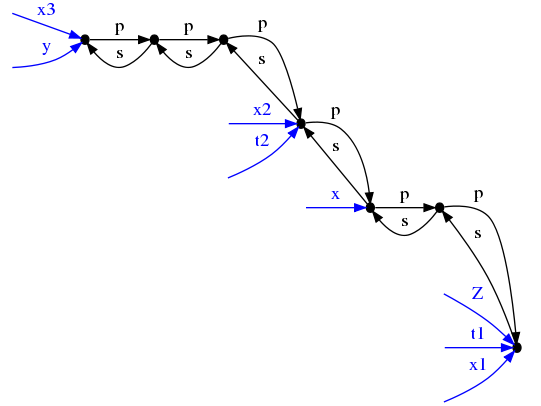
\includegraphics[scale=0.5]{fluid_2_2.png}

The source code of this assignment along with the programs can be found at
\url{github.com/comco/concurrency-theory-assignments}.
\end{document}
